\documentclass[handout]{beamer}
\usepackage{pgfpages}
\pgfpagesuselayout{4 on 1}[border shrink=2mm]
\usetheme{Copenhagen}
\usepackage{tikz}

\title{Beamer Presentations}
\date{}
\author{Gary}

\begin{document}
\maketitle

\section{Outline}
\begin{frame}
	\tableofcontents
\end{frame}

\section{Introduction}\label{introduction}

\begin{frame}
This is a sentence...
\begin{itemize}
	\item Hello
	\item Goodbye
	\item Apple 
\end{itemize}
\end{frame}

\begin{frame}{This is a detailed topic}
	content...
\end{frame}

\begin{frame}{Blocks}
	\begin{block}{An interesting observation}
		A more detailed discussion of what was observed. \\
		More text
	\end{block}
A smaller topic
\end{frame}

\begin{frame}{Alert Block}
	\begin{alertblock}{Alert!!!}
		Don`t yell at students!
	\end{alertblock}
\end{frame}

\begin{frame}
	\begin{example}
		This is a quick example. 
	\end{example}
\end{frame}

\begin{frame}{Definitions}
	\begin{definition}
		X is always equal to 7. 
	\end{definition}
\end{frame}

\section{Methods}
\begin{frame}
	\begin{itemize}
		\item<alert@1> Item 1
		\item<alert@2> Item 2
		\item<alert@3> Item 3
	\end{itemize}
\end{frame}

\begin{frame}\label{cat}
\begin{columns}
	\column {0.5\textwidth}
	This is a sample sentence. \\
	Another line
	\column {0.5\textwidth}
	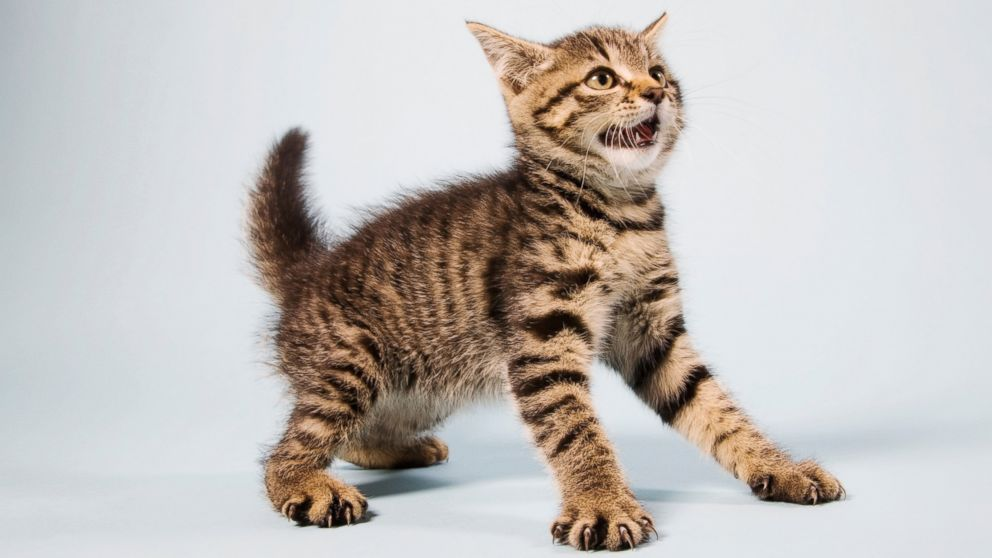
\includegraphics[width=5cm]{Figures/cat}
\end{columns}
\end{frame}

\begin{frame}
\frametitle{Using Columns and Table}
\begin{columns}
	\column{0.5\textwidth}
	This is some sample text with a table. 
	\column{0.5\textwidth}
	\begin{table}[]
		\centering
		\resizebox{\textwidth}{!}{%
			\begin{tabular}{llll}
				\hline
				Charachteristics & IoT & Edge & Cloud \\ \hline
				Deployment & Distributed & Distributed & Centralised \\
				Components & Physical Devices & Edge nodes & Virtual  \\
				Computational & Very Limited & Limited & Unlimited \\
				Storage & Small & Limited & Unlimited \\
				Response Time & NA & Fast & Slow \\
				Big Data & Source & Process & Process \\
				QoS & NA & High & Medium \\
				Energy  & Low & Low & High \\
				\hline
			\end{tabular}
		}
		\caption{Layer Characteristics}
		\label{tab:reasoning_layers}
	\end{table}
\end{columns}
\end{frame}

\begin{frame}
\frametitle{Using Columns and Tikz}
\begin{columns}
	\column{0.5\textwidth}
	This is some sample text with a Tikz plot. 
	\column{0.5\textwidth}
	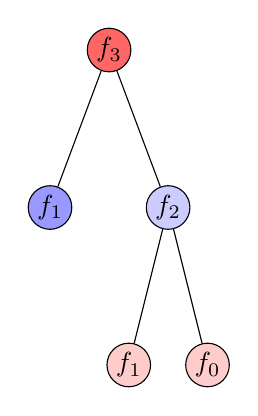
\begin{tikzpicture}
	[level distance=20mm%
	,every node/.style={fill=red!60,%
		circle,%
		draw=black,%
		inner sep=1pt}%
	,level 1/.style={sibling distance=15mm},%
	,level 2/.style={sibling distance=10mm,%
		nodes={fill=red!20}}]
	\node (top) {$f_3$}
	child {node[fill=blue!40] {$f_1$}}
	child {node[fill=blue!20] {$f_2$}
		child {node {$f_1$}}
		child {node {$f_0$}}};
	\end{tikzpicture}
\end{columns}
\end{frame}

\begin{frame}
\frametitle{There is No Largest Prime Number}
\framesubtitle{The Proof Uses \emph{Reductio ad Absurdum}}
\begin{proof}
	\begin{enumerate}
		\item<alert@2> Suppose the number of primes is finite.
		\item<alert@3> Let $p$ be the product of all primes.
		\item<alert@4> Then $p + 1$ is not divisible by any prime.
		\item<alert@5> Therefore, $p + 1$ is also a prime.
		\qedhere
	\end{enumerate}
\end{proof}
\end{frame}

\section{Results}\label{results}
\begin{frame}
\frametitle{Tables}
\begin{table}
	\begin{tabular}{|l|c|c|c|c|}
		\hline
		Competitor Name & Swim & Cycle & Run & Total \\ \hline
		John T & 13:04 & 24:15 & 18:34 & 55:53 \onslide<2-> \\ 
		Norman P & 8:00 & 22:45 & 23:02 & 53:47 \onslide<3->\\
		Alex K & 14:00 & 28:00 & n/a & n/a \onslide<4->\\
		Sarah H & 9:22 & 21:10 & 24:03 & 54:35 \\ \hline
	\end{tabular}
	\caption{Triathlon results}
\end{table}
\end{frame}

\begin{frame}{Hyperlinks}
\hyperlink{cat}{\beamerbutton{Cat Picture}}
\hyperlink{introduction}{\beamerreturnbutton{Introduction}}
\hyperlink{results}{\beamergotobutton{Results}}
\end{frame}

\begin{frame}[b]
content...
\end{frame}












\end{document}